\documentclass[12pt]{jarticle}
\usepackage[dvipdfmx]{graphicx}
\usepackage{url}
\usepackage{listings,jlisting}
\usepackage{ascmac}
\usepackage{amsmath,amssymb}

%ここからソースコードの表示に関する設定
\lstset{
  basicstyle={\ttfamily},
  identifierstyle={\small},
  commentstyle={\smallitshape},
  keywordstyle={\small\bfseries},
  ndkeywordstyle={\small},
  stringstyle={\small\ttfamily},
  frame={tb},
  breaklines=true,
  columns=[l]{fullflexible},
  numbers=left,
  xrightmargin=0zw,
  xleftmargin=3zw,
  numberstyle={\scriptsize},
  stepnumber=1,
  numbersep=1zw,
  lineskip=-0.5ex
}
%ここまでソースコードの表示に関する設定

\title{知能プログラミング演習II 課題5}
\author{グループ8\\
  29114003 青山周平\\
}
\date{2019年11月25日}

\begin{document}
\maketitle

\paragraph{提出物} work5
\paragraph{グループ} グループ8
\paragraph{メンバー}
\begin{tabular}{|c|c|c|}
  \hline
  学生番号&氏名&貢献度比率\\
  \hline\hline
  29114003&青山周平&20\\
  \hline
  29114060&後藤拓也&20\\
  \hline
  29114116&増田大輝&20\\
  \hline
  29114142&湯浅範子&20\\
  \hline
  29119016&小中祐希&20\\
  \hline
\end{tabular}

\section{課題の説明}
\begin{description}
\item[必須課題5-1] 目標集合を変えてみたときに,動作が正しくない場合があったかどうか,実行例を示して考察せよ.
また,もしあったならその箇所を修正し,どのように修正したか記せ.
\item[必須課題5-2] 教科書のプログラムでは,オペレータ間の競合解消戦略としてランダムなオペレータ選択を採用している.
これを,効果的な競合解消戦略に改良すべく考察し,実装せよ.
改良の結果,性能がどの程度向上したかを定量的に(つまり数字で)示すこと.
\item[必須課題5-3] 上記のプランニングのプログラムでは,ブロックの属性(たとえば色や形など)を考えていないので,色や形などの属性を扱えるようにせよ.ルールとして表現すること.
例えば色と形の両方を扱えるようにする場合,Aが青い三角形,Bが黄色の四角形,Cが緑の台形であったとする.
その時,色と形を使ってもゴールを指定できるようにする("green on blue" や"blue on box"のように)
\item[必須課題5-4] 上記5-2, 5-3で改良したプランニングシステムのGUIを実装せよ.
ブロック操作の過程をグラフィカルに可視化し,初期状態や目標状態をGUI上で変更できることが望ましい.
\item[発展課題5-5] ブロックワールド内における物理的制約条件をルールとして表現せよ.
例えば,三角錐(pyramid)の上には他のブロックを乗せられない等,その世界における物理的な制約を実現せよ.
\item[発展課題5-6] ユーザが自然言語(日本語や英語など)の命令文によってブロックを操作したり,初期状態/目標状態を変更したりできるようにせよ.
なお,命令文の動詞や語尾を1つの表現に決め打ちするのではなく,多様な表現を許容できることが望ましい.
\item[発展課題5-7] 3次元空間 (実世界) の物理的な挙動を考慮したブロックワールドにおけるプランニングを実現せよ.
なお,物理エンジン等を利用する場合,Java以外の言語のフレームワークを使って実現しても構わない.
\item[発展課題5-8] 教科書3.3節のプランニング手法を応用できそうなブロック操作以外のタスクをグループで話し合い,新たなプランニング課題を自由に設定せよ.
さらに,もし可能であれば,その自己設定課題を解くプランニングシステムを実装せよ.
\end{description}

\section{必須課題5-4}
\begin{screen}
上記5-2, 5-3で改良したプランニングシステムのGUIを実装せよ.
ブロック操作の過程をグラフィカルに可視化し,初期状態や目標状態をGUI上で変更できることが望ましい.
\end{screen}
私の担当箇所は,必須課題5-4におけるGUIとPlanner.javaとの間でデータの仲介を行うPresenterの制作である.

\subsection{手法}
Presenterを実装するにあたり,以下のような方針を立てた.
\begin{enumerate}
\item Planner.javaのデータを,外部から取り出し,セットできるように改良する.
\item 導かれたプランの導出過程を渡せるようにする.
\end{enumerate}

1.に関して,MVPアーキテクチャを導入し,GUIとPlanner間のデータのやり取りを,Presenterによって緩衝することで,拡張性の向上とGUI担当者の負担軽減を図った.

2.に関して,GUI担当者が受け取りやすい渡し方を相談して決めることで,柔軟に対応した. \\

\subsection{実装}
Presenter.javaには以下のクラスが含まれる.
\begin{description}
\item[Presenter] テスト用のmainメソッド,擬似的な各種のゲッタやセッタ,導出過程をPlannerから取得するメソッド等を実装したクラス.
\end{description}

\subsubsection{Planner.javaのデータを,外部から取り出し,セットできるように改良する.}
初期化をコンストラクタで行わせたり,クラスフィールドに値を移行したりすることで実現した.

\subsubsection{導かれたプランの導出過程を渡せるようにする.}
得られたplanを渡すために,Plannerクラス内にOperatorクラスのplanUnifiedResultフィールドを追加し,Operatorクラス内にHashMapクラスのbindingsフィールドを追加した.bindingsは変数束縛を示すものであり,getBindingsにより取得できるようにした.

具体的な渡し方としては,Plannerのプランニングにより得られたplanを,全オペレータとunifyして,当てはまるものがあったらunifyにより明らかになった変数束縛を引数に,新たなOperatorインスタンス生成し,planUnifiedResultに追加してplanUnifiedResultを渡すというものである.

この挙動をソースコード
\ref{pur}に示す.

\begin{lstlisting}[caption=Plannerクラスのstartメソッドの一部, label=pur]
  public void start() {
    ...
    planning(goalList, initialState, theBinding);

      System.out.println("***** This is a plan! *****");
      planResult = new ArrayList<>();
      planUnifiedResult  = new ArrayList<>();
      for (int i = 0; i < plan.size(); i++) {
        Operator op = (Operator) plan.get(i);
        Operator result = (op.instantiate(theBinding));
        System.out.println(result.name);
        planResult.add(result.name);
        for(Operator initOp : operators) {
          Unifier unifier = new Unifier();
          if(unifier.unify(result.name, initOp.getName())) {
            planUnifiedResult.add(new Operator(initOp, unifier.getVars()));
            break;
          }
        }
      }
    }
\end{lstlisting}

\subsection{実行例}
Presenter.javaのmainメソッドを実行したところ,以下のような結果が得られ,値が正しく取得できていることが分かる.

\begin{lstlisting}[caption=Presenterの実行, label=pres]
...
***** This is a plan! *****
pick up B from the table
...

-----on Presenter-----
[clear blue, clear green, clear red, ontable ball, ontable trapezoid, ontable box, ontable pyramid, handEmpty]
[trapezoid on box, ball on trapezoid]
pick up ?x from the table
{?x=B}
\end{lstlisting}

\subsection{考察}
今回のPresenterは特にやることがなく,GUI側の負担が大きいように感じた.しかし,GUI制作経験のある身として,可能な限りGUIが扱いやすいようなPresenterとなるよう心がけた.例えば,プランの過程の渡し方は,Operatorを少し書き加えて実現したことで,変数束縛も簡単に一緒に取得できるようにしたことや,String型でも過程を受け取れるようにしたことでGUI側で行うべき処理を減らせるようにしたことである.

しかし,今回の課題も前回同様最初はどのような形で値を渡すかで悩むこととなった.前回よりも早く意識のすり合わせと進捗の説明を担当者間で共有できたため,今回はよりスムーズに実装に漕ぎ着けたのだと考えられる.

\section{発展課題5-7}
\begin{screen}
3次元空間 (実世界) の物理的な挙動を考慮したブロックワールドにおけるプランニングを実現せよ.
なお,物理エンジン等を利用する場合,Java以外の言語のフレームワークを使って実現しても構わない.
\end{screen}
私の担当箇所は,発展課題5-7におけるプランニングの,Unityを用いた実装である.

\subsection{手法}
3次元空間の物理的な挙動を考慮したブロックワールドにおけるプランニングを実現するにあたり,以下のような方針を立てた.
\begin{enumerate}
\item 空間やプランに関するオブジェクトを生成する.
\item プランニングを行えるようにスクリプトを作成する.
\end{enumerate}

1.に関して,物体を生成し,コンポーネントを付与することで物理的な挙動を行えるようにした.また,3種類のプランを実装することで,物理制約の確認を容易に行えるような仕様とした.

2.に関して,C\#スクリプトを用いてキーボードやマウスの入力を受け付けられるように実装した.Masterオブジェクトを作ってそこにアタッチすることで,それらの操作を一括的に管理できるような仕様とした.

\subsection{実装}
Mainシーンに含まれるオブジェクトには以下のものが含まれる.
\begin{description}
\item[Main Camera] 主カメラに関するオブジェクト.Room全体をやや見下ろし気味に映す.
\item[Directional Light] オブジェクト全体を照らす照明.
\item[Master] スクリプトをアタッチするための空オブジェクト.
\item[Room] 6個のPlaneオブジェクトを子に持つ,立方体の部屋を構成するオブジェクト.
\item[Cube] 直方体のブロックを生成するプレハブ.
\item[Sphere] 球のブロックを生成するプレハブ.
\item[Torus] 円環体のブロックを生成するプレハブ.
\end{description} 

C\#スクリプトでは以下のものが実装されている.
\begin{description}
\item[Clicked] クリックされたオブジェクトにフォーカスを当てるスクリプト.
\item[Operationg] Clickedでフォーカスされたオブジェクトにキーボード入力を反映するスクリプト.
\item[Generator] キーボード入力に合わせてブロックを生成するスクリプト.
\item[Destroyer] クリックされたオブジェクトを削除するためのスクリプト.
\end{description}

\subsubsection{空間やプランに関するオブジェクトを生成する.}
まず,オブジェクトの受け皿となる部屋の実装を行った.オブジェクトにはPlaneを用い,コンポーネントMesh Colliderをアタッチすることで,ブロックとの衝突判定を実現した.Planeオブジェクトの特徴として,裏面からはオブジェクトが透明に見えることが挙げられる.これにより,外部から可視化した状態のまま密閉空間を実現できた.

次に,CubeやSphereのオブジェクトを用いてプレハブの元となる直方体と球のブロックを実装した.直方体にはBox Collider,球にはSphere Colliderをアタッチすることで衝突判定を実現し,更にいずれに対してもPigidbodyをアタッチすることで,質量や重力に関する挙動を実現し,より物理的な挙動を考慮したプランニングが実現できるようになった.また,Physic Materialを作成し各ブロックのColliderにアタッチすることで,摩擦も考慮した挙動が実現できた.そしてこれらのオブジェクトはプレハブにすることで,同オブジェクトの複製が容易に行えるようになった.

次に,球ブロックの受け皿として最適だと思い,円環体のブロックの実装を試みた.しかし直方体や球とは異なり,プリミティブなゲームオブジェクトからでは実装は難しかったため,PackageManagerに含まれる機能である,ProBuilderを用いて実装を試みた.これにより円環体の生成はできたものの,形が複雑であるため,衝突判定にはMesh Colliderを用いる必要があった.

しかし,Mesh Colliderは他のオブジェクトとの衝突判定を無視したり,設定を弄って衝突判定が行われるようになっても内側の穴が穴としての判定がなされなかったりと,その挙動に悩まされることとなった.

そこで,円環体の衝突判定にはAsset StoreからSAColliderBuilderをインポートし,それを用いることにした.SAColliderBuilderのコンポーネントSAMeshColliderBuilderからSplit Polygon Normalをオンにし,Shape TypeをMeshに,Mesh TypeをConvex Hullにすることで,Rigidbodyとしての挙動を残したまま,穴を含む正確な衝突判定を実現できた.

しかしこれをプレハブ化すると,SAColliderBuilderが正常な挙動がなされず,再度床をすり抜けるようになってしまった.設定を弄っていると''Non-convex MeshCollider with non-kinematic Rigidbody is no longer supported since Unity 5.''といったエラーが出たことから,MeshColliderとRigidbodyは相性が悪いと考えられたため,そもそも円環体の当たり判定の方法を変えることにした.

判定にはSphere Colliderを組み合わせて行い,円環体の子オブジェクトとして衝突用のオブジェクトを持たせた.

SAColliderBuilderで実装した改良前の衝突判定と,Sphere Colliderを組み合わせで実装した改良後の衝突判定を
図\ref{fig:bwp1}と図\ref{fig:bwp2}に示す.

\begin{figure}[!hbt]
  	\begin{center}
  		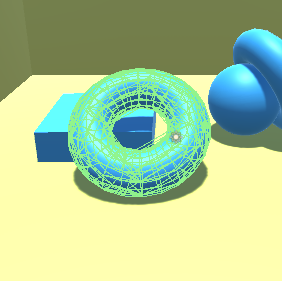
\includegraphics[scale=0.55]{images/bwp1.png}
	\end{center}
  	\caption{改良前}
  	\label{fig:bwp1}
\end{figure}

\begin{figure}[!hbt]
  	\begin{center}
  		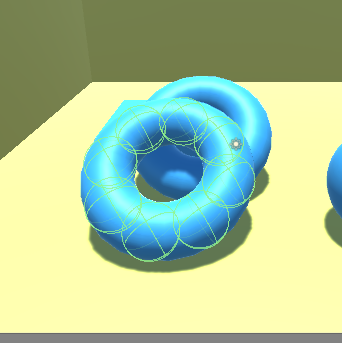
\includegraphics[scale=0.5]{images/bwp2.png}
	\end{center}
  	\caption{改良後}
  	\label{fig:bwp2}
\end{figure}

このように,円環体の当たり判定が簡略されながらも充分に実現されていることが分かる.Sphere Colliderで実現したことにより,プレハブ化してもRigidbodyとの併用が問題なく行うことができた.

\subsubsection{プランニングを行えるようにスクリプトを作成する.}
Clicked.csについて,クリックされたときにまずフォーカス対象のオブジェクトをnullにしている.次にクリックしたオブジェクトの取得をRaycastを用いて行うが,操作対象外の床等のオブジェクトをフォーカス対象外にする必要があった.これはフォーカス対象のブロックにPlanというタグを統一して付けることで,CompareTagからその判定を行えるようにした.また,円環体の当たり判定である子オブジェクトをクリックで検出したとき,親オブジェクトを取り扱うように,rootフィールドを用いてその値を取得した.

クリックしたときに実行されるUpdateメソッドは以下のとおりである.

\begin{lstlisting}[caption=ClickedクラスのUpdateメソッド, label=clicked]
    void Update()
    {
        if (Input.GetMouseButtonDown(0))
        {
            if(clickedGameObject != null)
            {
                clickedGameObject = null;
            }

            Ray ray = Camera.main.ScreenPointToRay(Input.mousePosition);
            RaycastHit hit = new RaycastHit();

            if (Physics.Raycast(ray, out hit))
            {
                clickedGameObject = hit.collider.gameObject.transform.root.gameObject;  // 親要素の取得
                if (!clickedGameObject.CompareTag("Plan"))
                {
                    clickedGameObject = null;  // Planeは対象外
                }
            }

            Debug.Log(hit.collider.gameObject);
        }
    }
\end{lstlisting}

Operating.csでは,Clickedクラスで取得したオブジェクトの移動のために,GetKeyメソッドを用いてキーボードの入力判定を行った.初めはスクリプト内で一時的に対象のオブジェクトのRigidbodyのisKinematicをtrueにしてtransformのpositionにVector3を足し合わせることで移動させていたが,それだと摩擦の判定が行われなかったり,衝突判定を貫通して移動できてしまったりという問題があった.これはisKinematicをtrueにしたことが原因であると分かった.そこで,positionに足し合わせるのではなくAddForceでVector3を足し合わせるようにしたことで,isKinematicをfalseのまま物理的制約に準じた物体の移動を実現することが出来た.

キーボード入力時に挙動を示すOperatingクラスは以下の様になっている.

\begin{lstlisting}[caption=Operatingクラス, label=operating]
public class Operating : MonoBehaviour
{
    private Vector3 velocity;
    private float moveSpeed = 1000.0f;

    void Update()
    {
        velocity = Vector3.zero;
        if (Input.GetKey(KeyCode.W))
            velocity.z += 1;
        if (Input.GetKey(KeyCode.A))
            velocity.x -= 1;
        if (Input.GetKey(KeyCode.S))
            velocity.z -= 1;
        if (Input.GetKey(KeyCode.D))
            velocity.x += 1;
        if (Input.GetKey(KeyCode.E))
            velocity.y += 1;
        if (Input.GetKey(KeyCode.Q))
            velocity.y -= 1;
        // 速度ベクトルの長さを1秒でmoveSpeedだけ進むように調整します
        velocity = velocity.normalized * moveSpeed * Time.deltaTime;

        if (velocity.magnitude > 0)
        {
            // プレイヤーの位置(transform.position)の更新
            // 移動方向ベクトル(velocity)を足し込みます
            GameObject go = Clicked.clickedGameObject;
            if (go != null)
            {
                go.GetComponent<Rigidbody>().AddForce(velocity);
            }
        }
    }
}
\end{lstlisting}

Generator.csでは,ResourcesクラスのLoadメソッドからプレハブを取得し,Instantiateで生成するようにすることで,任意のタイミングで好きなだけブロックの生成ができるようにした. \\

Destroyer.csでは,Clicked.cs同様にタグを用いて判定することで,ブロック以外のオブジェクトが誤って消えることのないようにした. \\

また,これらのスクリプトは各オブジェクトにアタッチせずとも,Masterオブジェクトにさえアタッチすれば全体の挙動が管理できるような仕様としたことで,各オブジェクトに対する負荷を減らし,効率的なプログラムを実装することができた.

\clearpage

\subsection{実行例}
Block World Planning.exeを起動したところ,下図のような画面が得られる.

\begin{figure}[!hbt]
  	\begin{center}
  		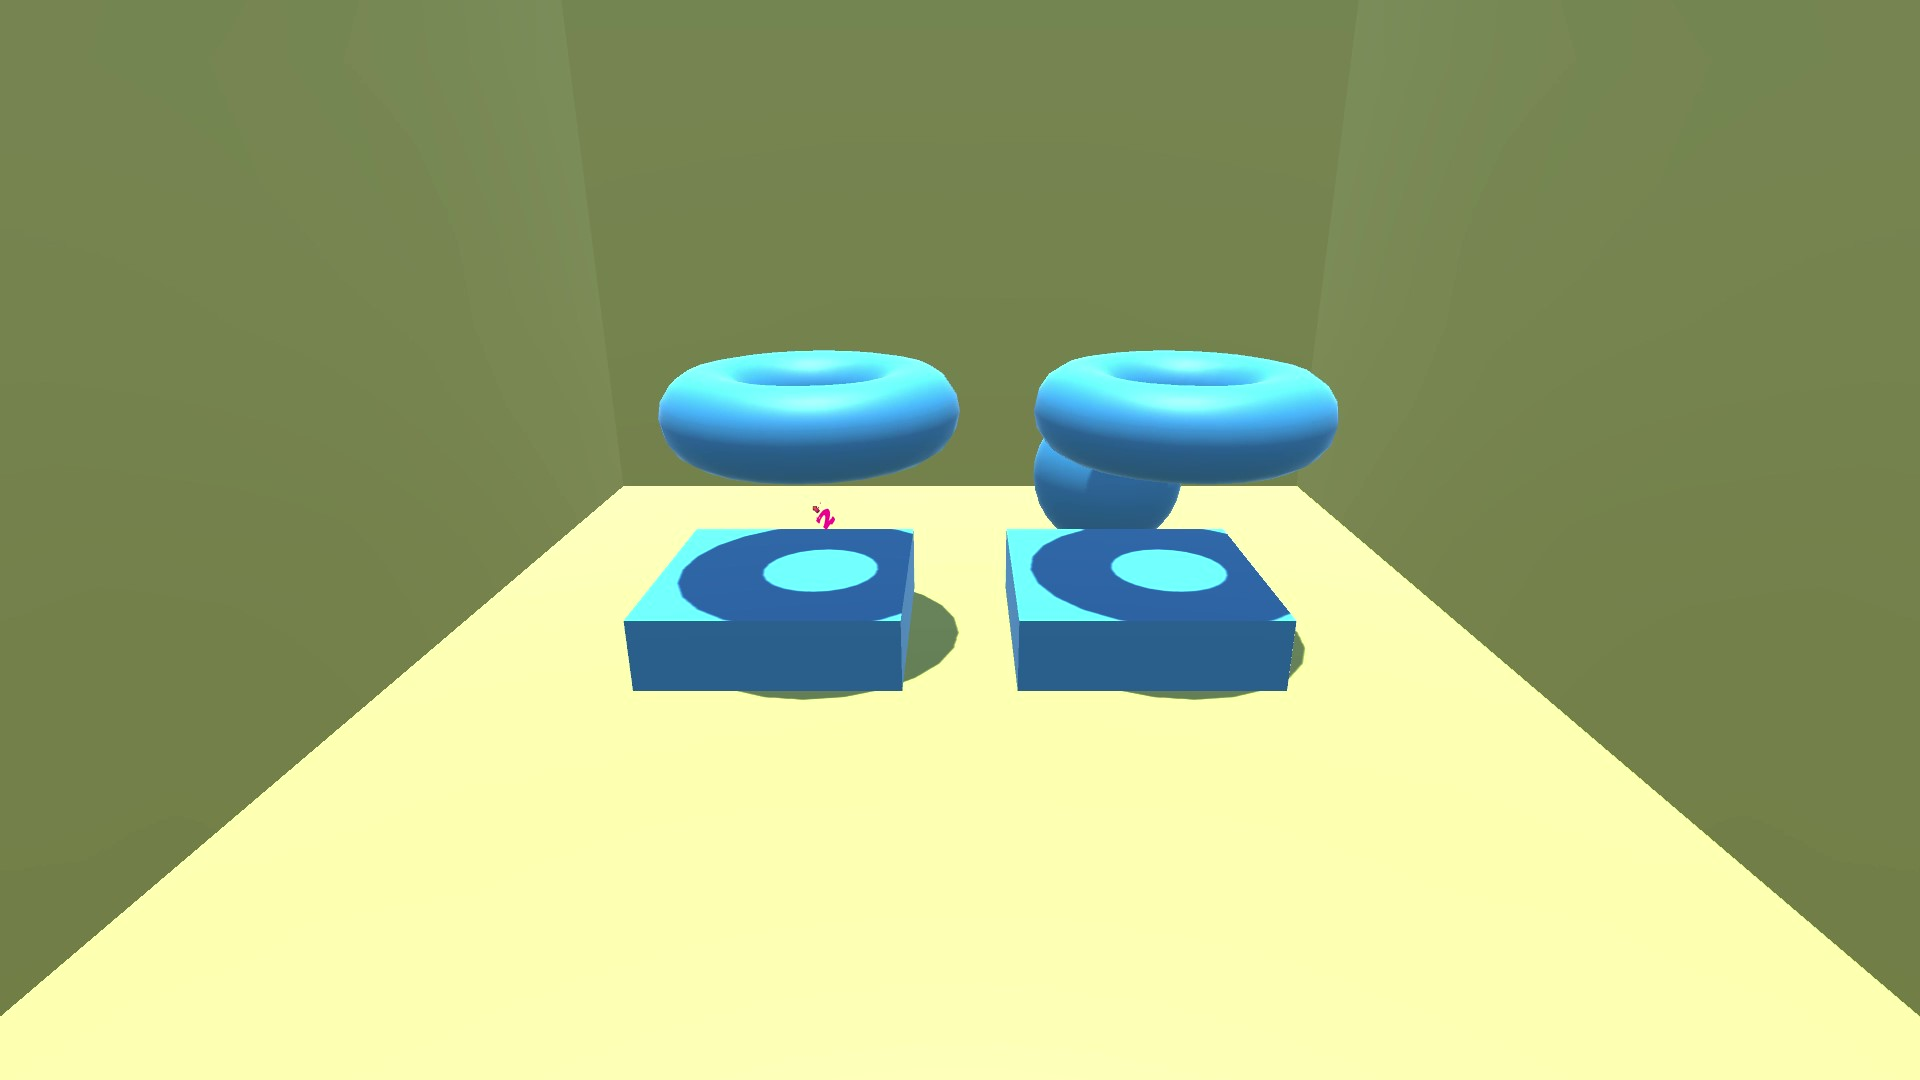
\includegraphics[scale=0.2]{images/bwp3.jpg}
	\end{center}
  	\caption{起動時の画面}
\end{figure}
\clearpage

右クリックでオブジェクトを削除でき,キー``1''で直方体,キー``2''で円環体,キー``3''で球のブロックを生成できる.これによって構成した下図をプランニングの初期状態とする.

\begin{figure}[!hbt]
  	\begin{center}
  		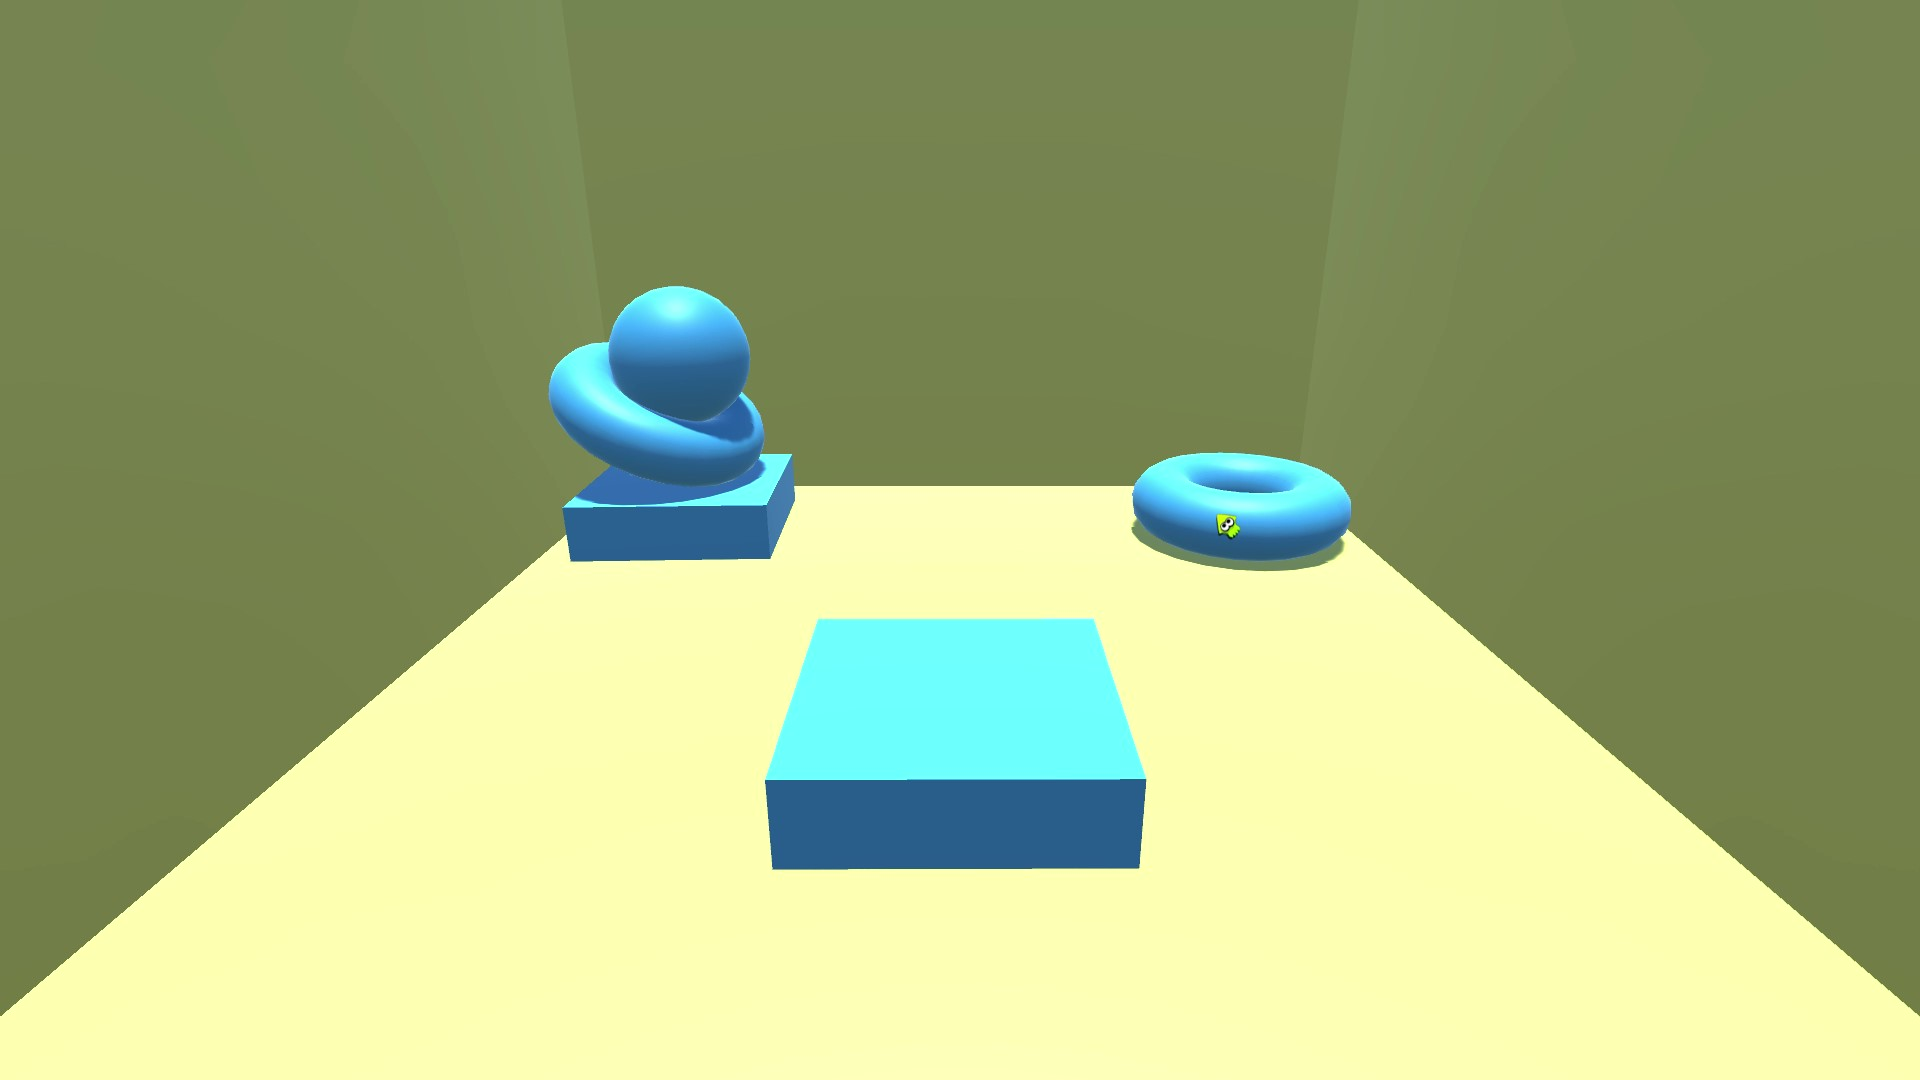
\includegraphics[scale=0.2]{images/bwp4.jpg}
	\end{center}
  	\caption{初期状態}
\end{figure}
\clearpage

左クリックで移動するオブジェクトを選択してから,WASDキーで上下左右,EQキーで昇降の移動が行える.手前の直方体に乗せるために右奥の円環体を持ち上げた様子が下図のとおりである.

\begin{figure}[!hbt]
  	\begin{center}
  		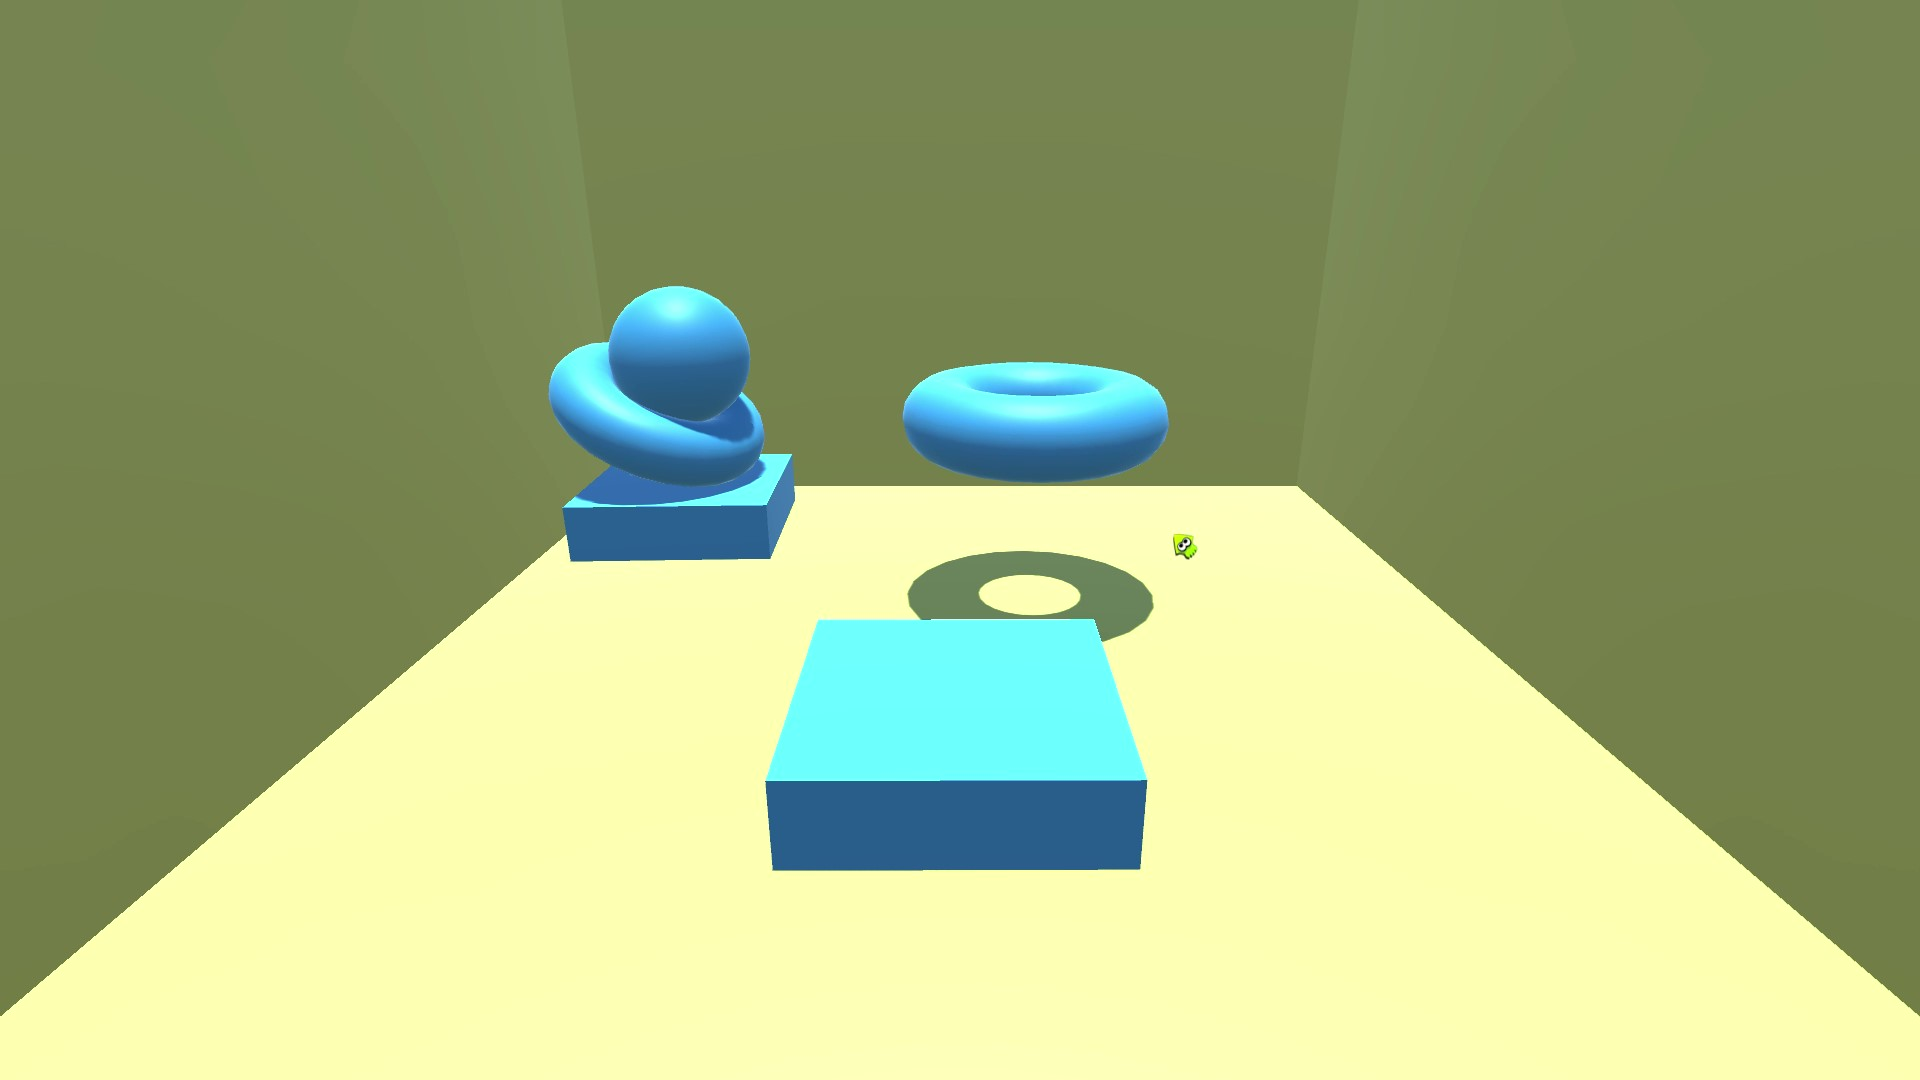
\includegraphics[scale=0.2]{images/bwp5.jpg}
	\end{center}
  	\caption{プランニング開始}
\end{figure}
\clearpage

そうして,物理的な挙動を考慮した上で円環体を直方体の上に乗せた様子が下図のとおりである.

\begin{figure}[!hbt]
  	\begin{center}
  		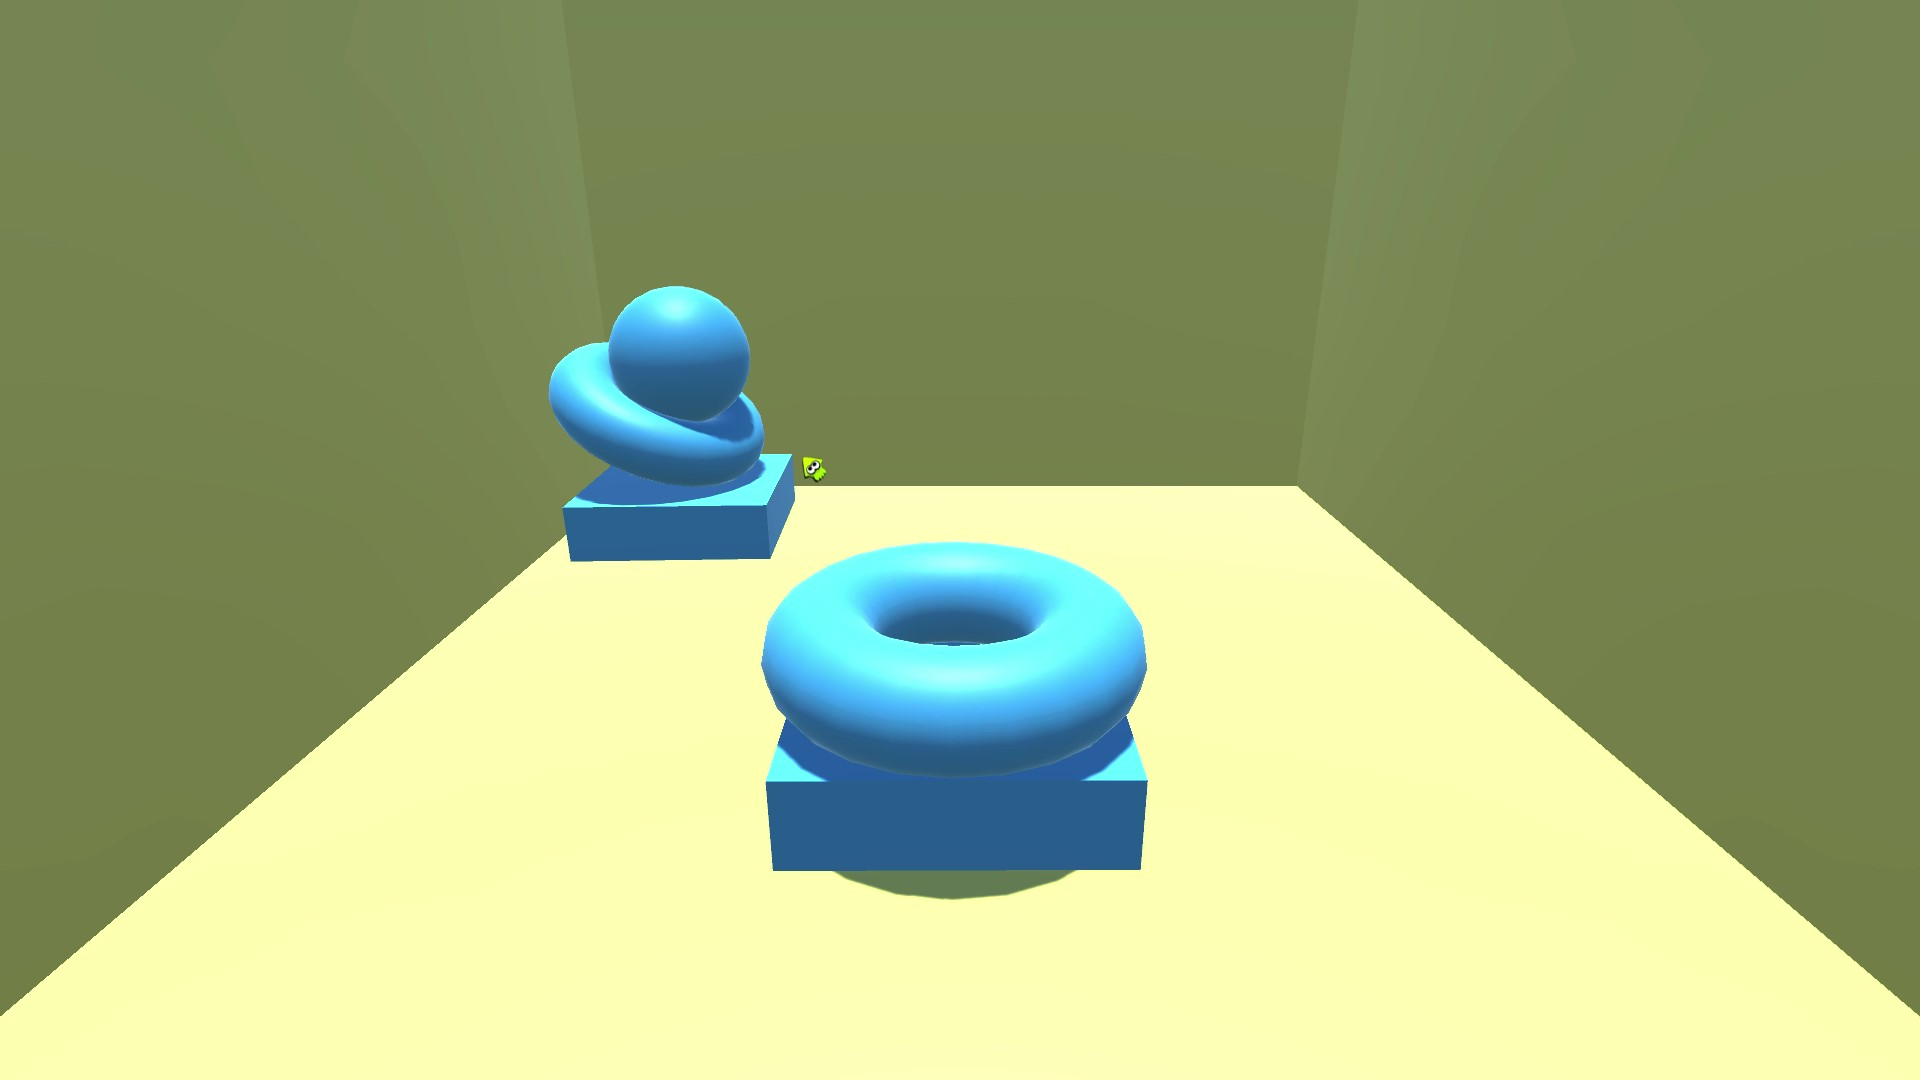
\includegraphics[scale=0.2]{images/bwp6.jpg}
	\end{center}
  	\caption{ステップ1完了}
\end{figure}
\clearpage

物理的な挙動を考慮して完了したプランニングが下図のとおりである.

\begin{figure}[!hbt]
  	\begin{center}
  		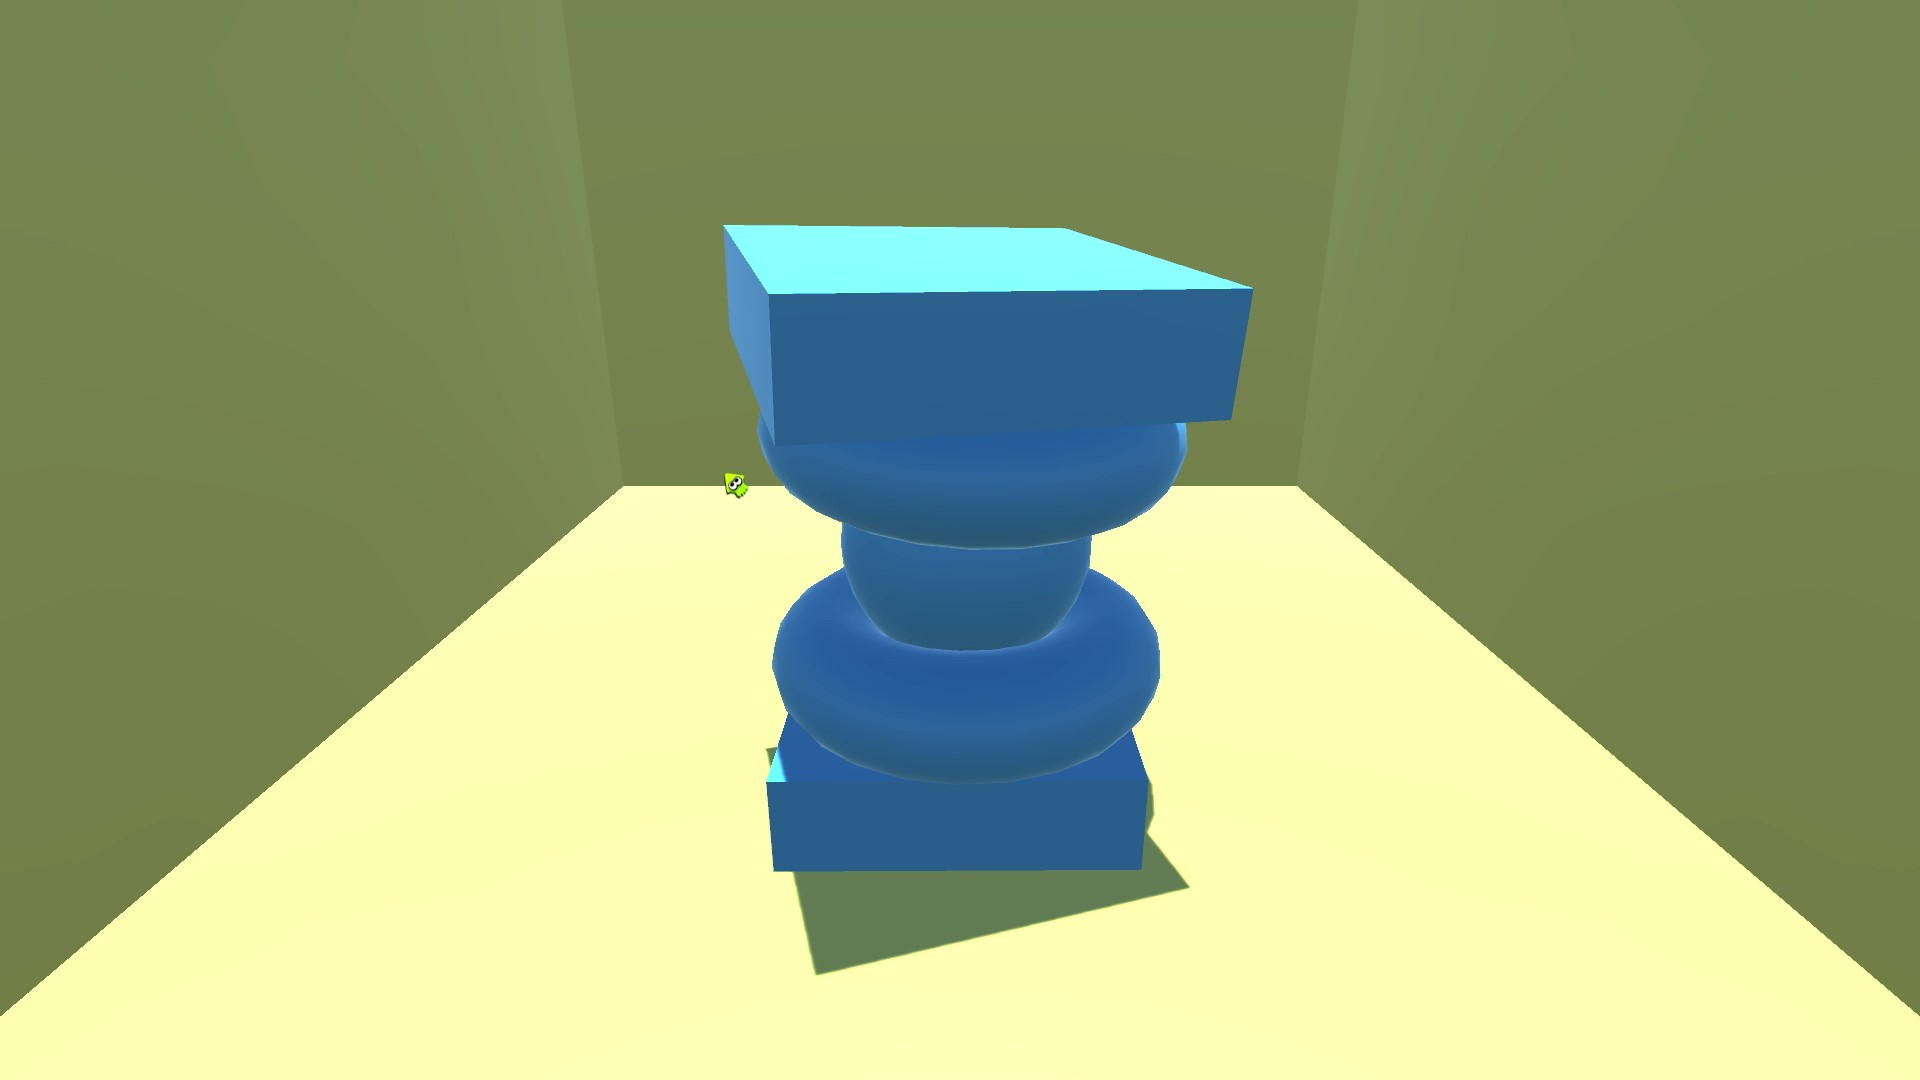
\includegraphics[scale=0.2]{images/bwp7.jpg}
	\end{center}
  	\caption{プランニング完了}
\end{figure}
\clearpage

\subsection{考察}
物理的な挙動を考慮したプランニングを実装するためにUnityを用いてみて,衝突判定や重力の考慮などを付けるだけなら容易に出来たが,円環体の穴の当たり判定が正しく設定できないなどで数多く躓いた.この問題はSphereColliderを工夫して用いることで解決したが,このように,実現したいものをマイナーなアセットを探して実現するのではなく,今ある機能を工夫して用いて実現する,という考え方は大切にすべきだと思った.

厳密な当たり判定が必要であったわけではなく,円環体の穴に自然な感じで球をはめたいというのが元々の目的であったことに気づいたおかげで解決できたように,本当に実現したいものは何か,本当に必要なものは何かを立ち返って考え,問題を簡略化することが,プログラミングの1つのテクニックであると考えられる. \\

また,子オブジェクトという概念に悩まされたように,UnityもJavaと同じ様に,ポインタが何を指しているかを考え,微妙な違いを見落とさないようにすることが重要であることを痛感した.UnityはJavaよりも並列的な処理がしやすい一方で,カプセル化に関しては大雑把な印象を受けたため,パブリックな変数がどのように遷移しているのか,Debug.Logをこまめに用いて確認することが大切だと思った. \\

また,Unityを使っていてフリーズやクラッシュが起こって,データが飛んだことがあった.Javaのプログラミングならそういうことが起こったことはないので,ゲームエンジンならではの重い処理の影響だと考えられる.このような普段と違うフレームワークを用いるときは,そのフレームワークに合わせてこまめにセーブをするといった対応や環境構築を行うことも大切だと考えられた.

\section{感想}
GUIもSwingじゃなくてUnityで作らせてもらえたらなあ.
でもSwingの経験も活きた.
javaプログラムのデータをどうUnityに渡すか.ファイル?


% 参考文献
\begin{thebibliography}{99}
Unity Technologies.: 『Unity - Manual: Unity User Manual (2019.2)』 https://docs.unity3d.com/Manual/index.html (2019/12/09アクセス) \\
\end{thebibliography}

\end{document}
